\section{\name Prototype}
\label{sec:prototype}

In this section we provide an overview of our \name prototype implementation.

\begin{figure}[t]
    \begin{center}
        \begin{subfigure}{0.4\textwidth}
        \centering
            %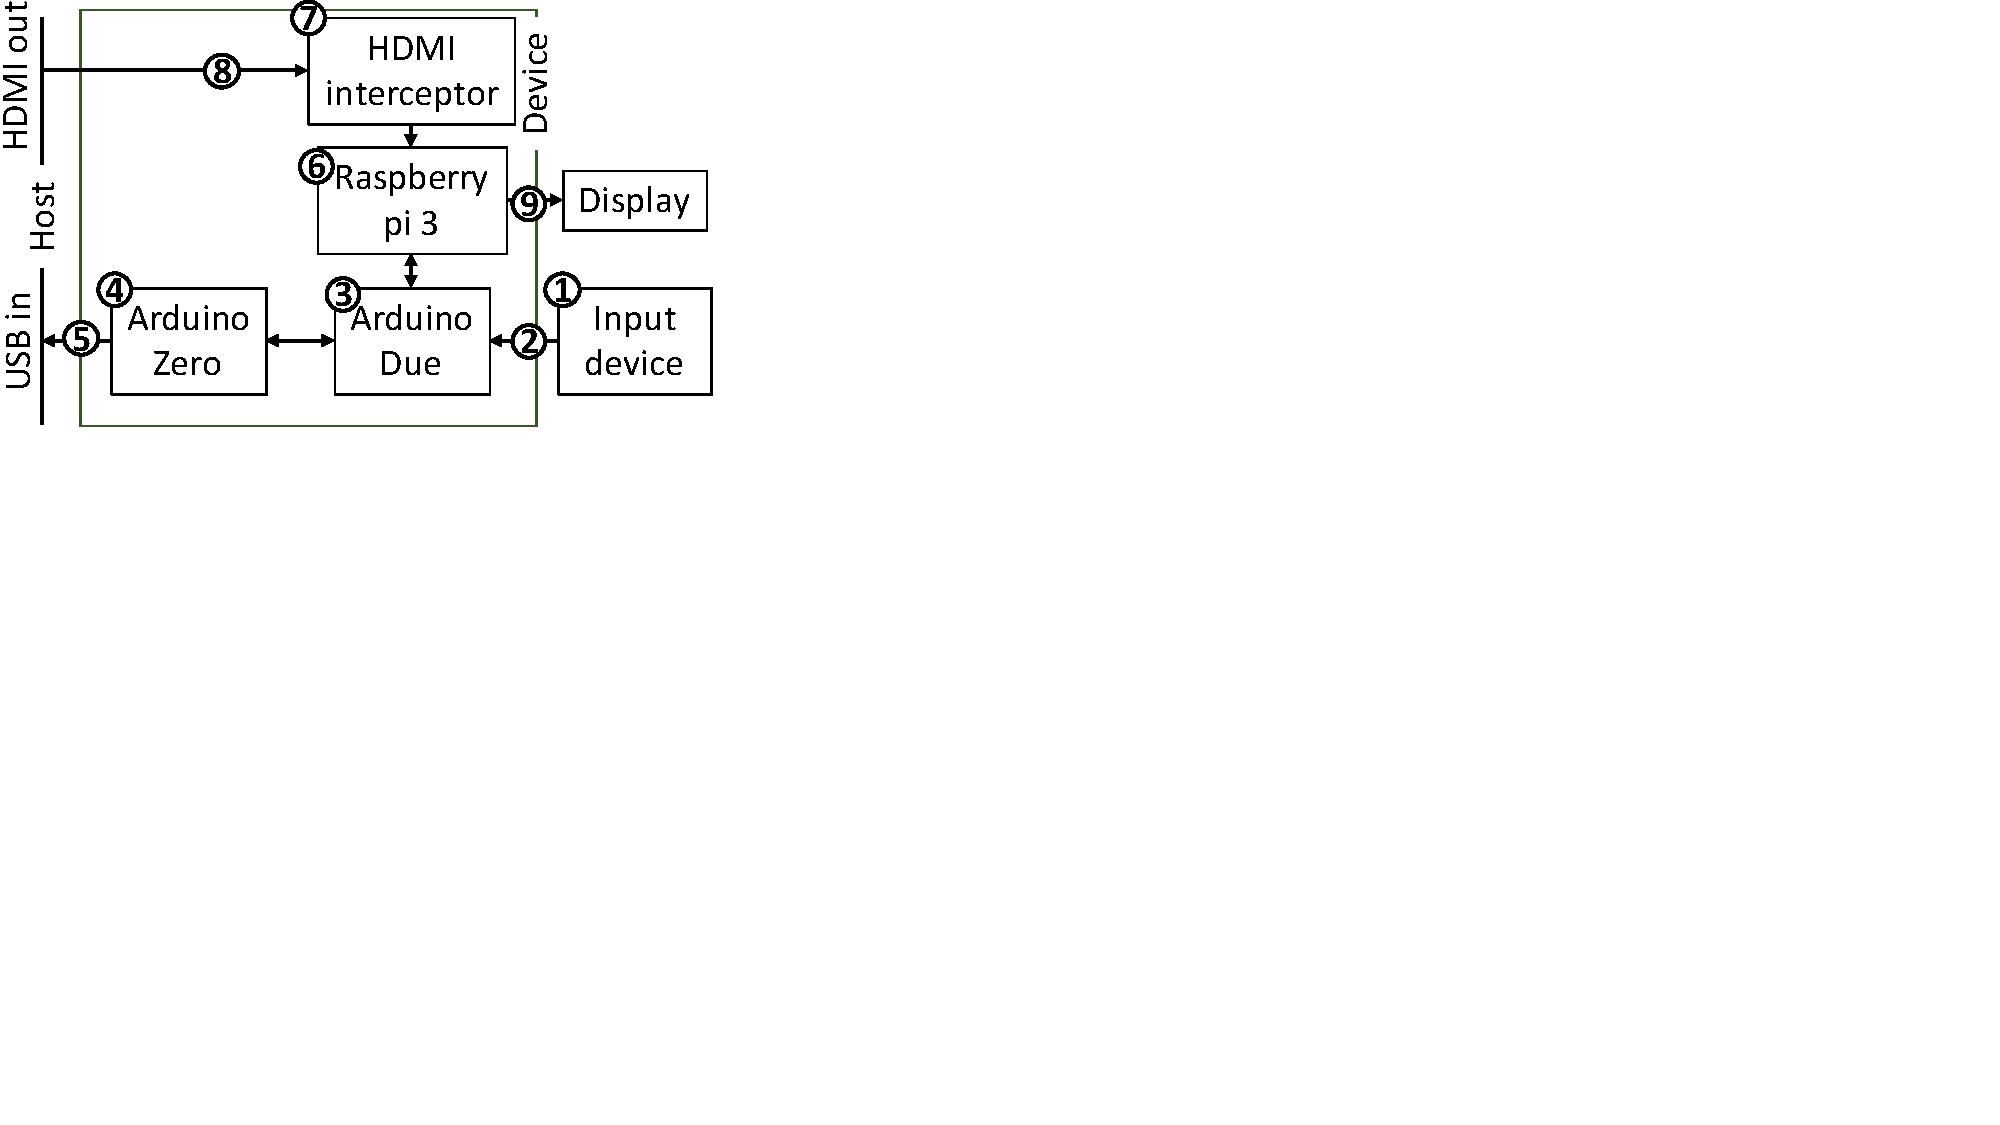
\includegraphics[trim={0 12cm 21.7cm 0}, clip, scale=0.45]{setUpBlock.pdf}
            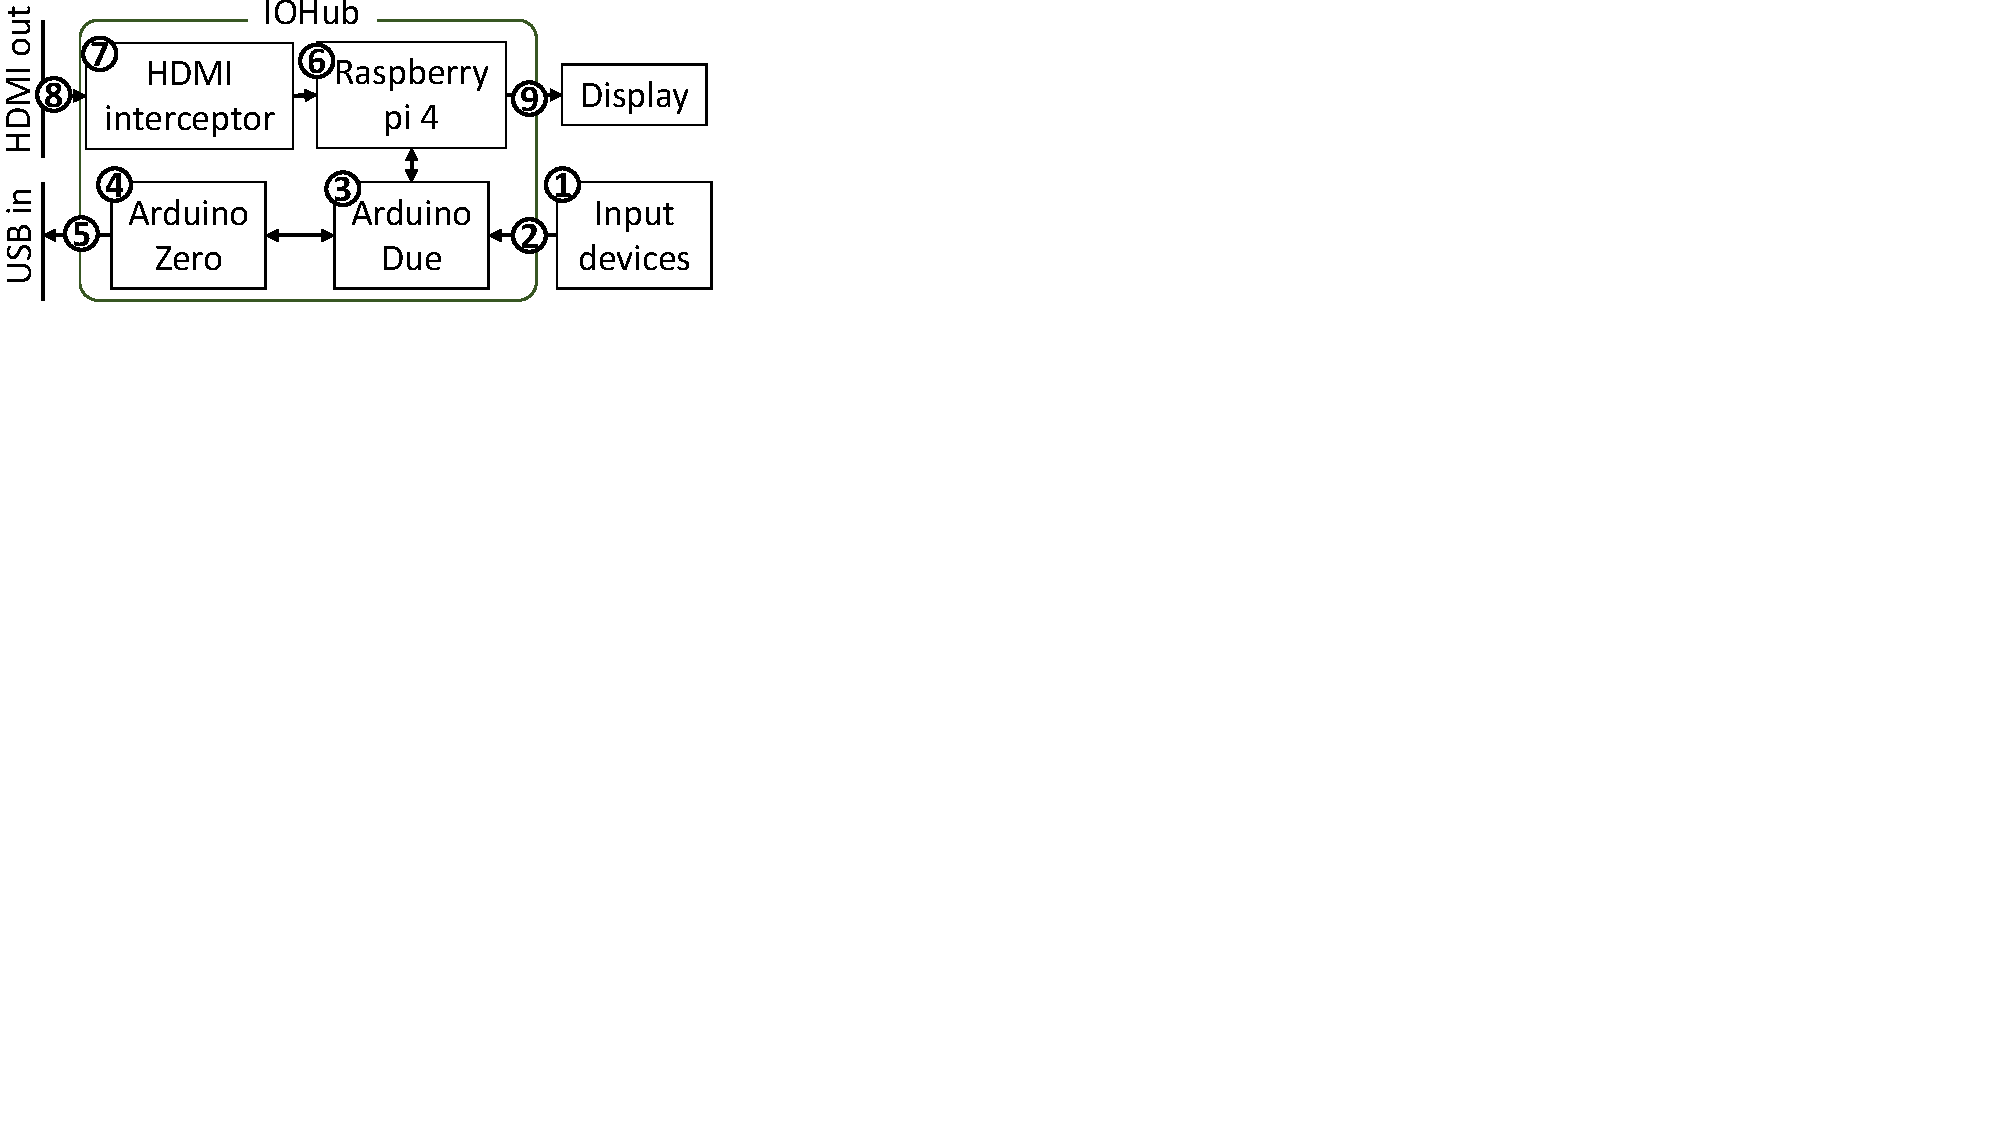
\includegraphics[trim={0 13.7cm 21.7cm 0}, clip, scale=0.4]{chapters/ProtectIOn/images/setUpBlock_1.pdf}
            \caption{The figure shows the basic components and connections between them in our \name prototype.}
            \label{fig:prototypeArch}    
        \end{subfigure}
    \end{center}
    
    %\vspace{1em} 
    
    \begin{center}
        \begin{subfigure}{0.4\textwidth}
        \centering
        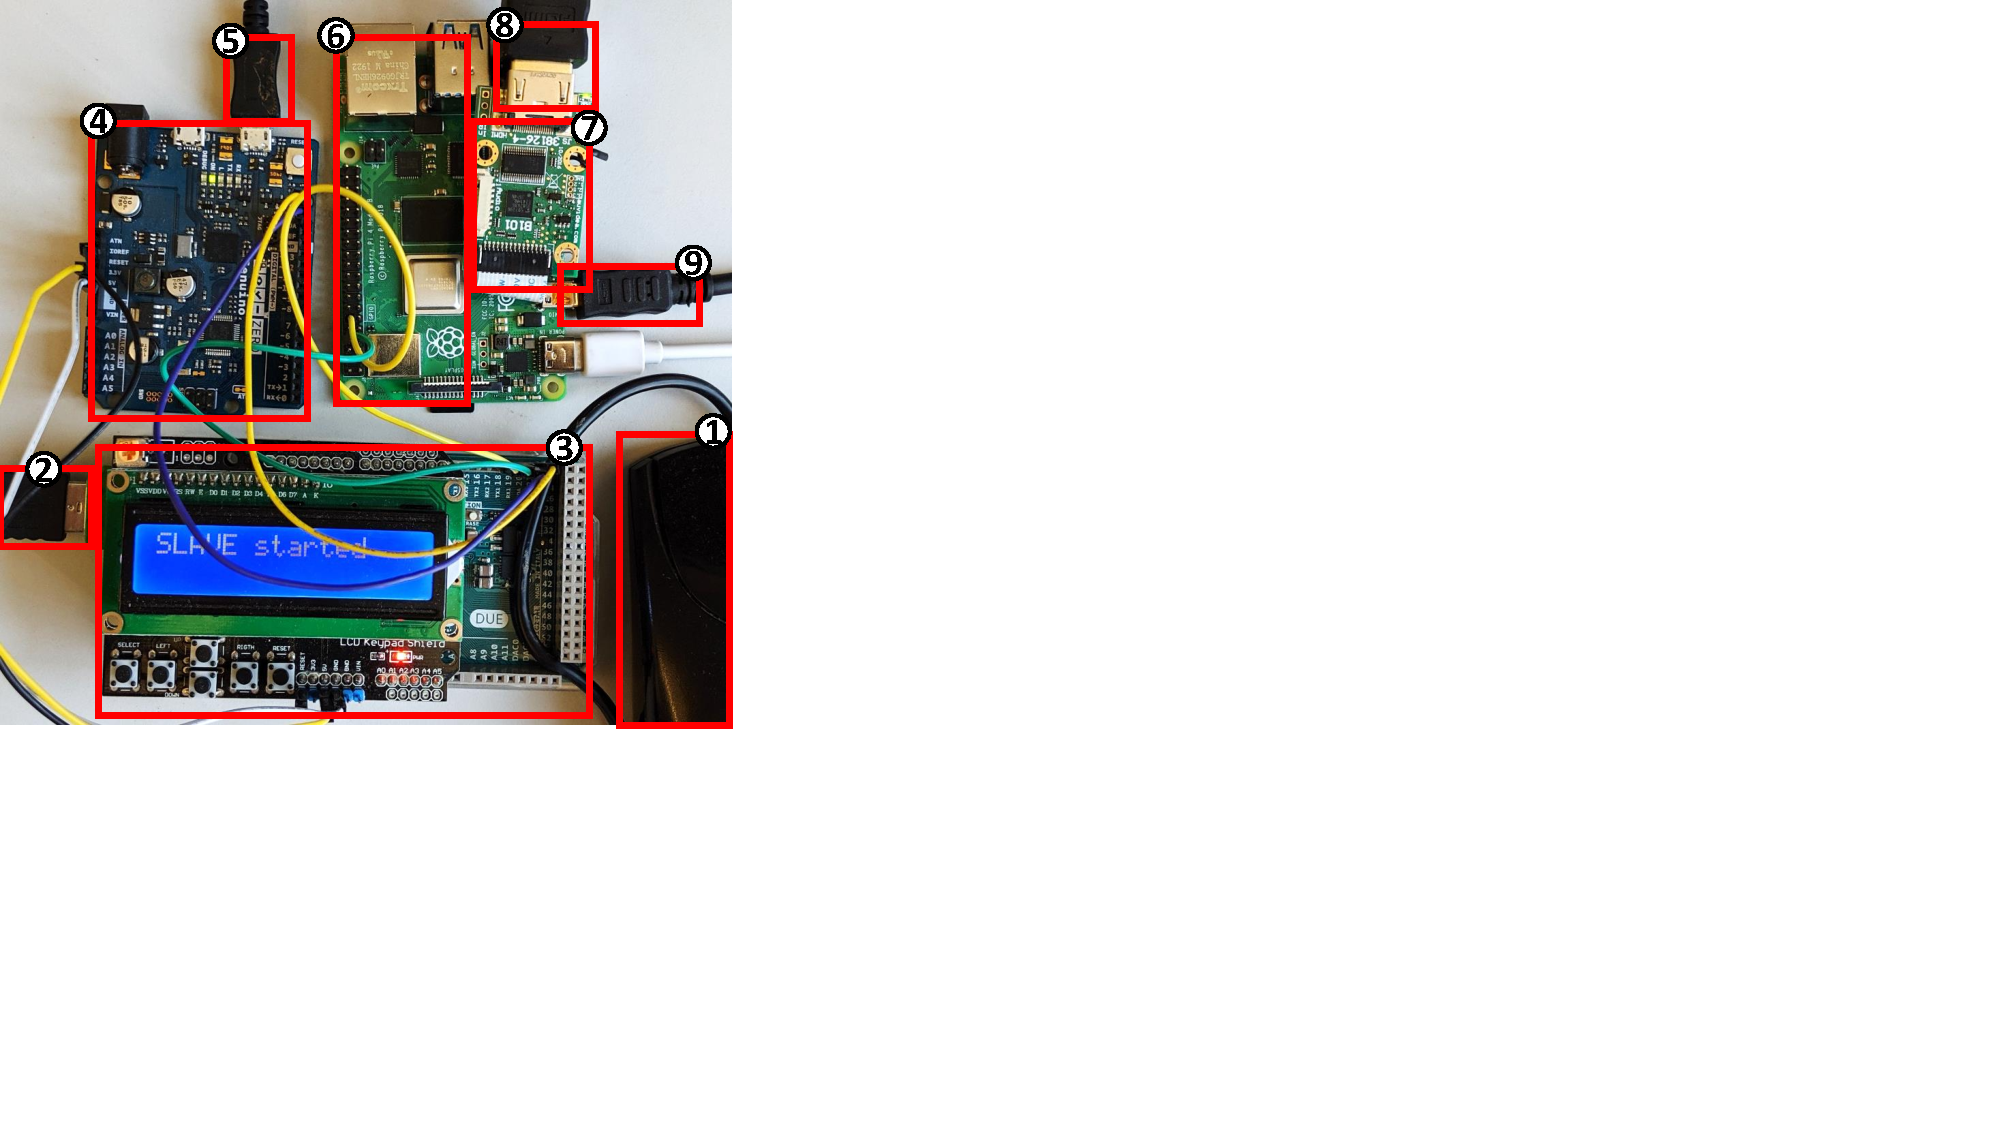
\includegraphics[trim={0 6.6cm 21.5cm 0}, clip, scale=0.5]{chapters/ProtectIOn/images/setUp_1.pdf}
        \caption{\name prototype uses Arduino Due and Zero microcontroller board and a Raspberry Pi 4 SBC. The highlighted numbers correspond to the labels in Figure~\ref{fig:prototypeArch}.}
        \label{fig:prototype}
    \end{subfigure}
    \end{center}
    
    \caption[\name prototype]{\textbf{\name prototype}. Figure~\ref{fig:prototypeArch} and~\ref{fig:prototype} shows the schematic and a photo of the  \name prototype respectively.} 
    \label{fig:prototypeAll}
    \spacesave
\end{figure}

\subsection{Setup} Here, we describe our prototype implementation of \name as an auxiliary device. Figure~\ref{fig:prototypeAll} depicts the \name prototype in two parts: Figure~\ref{fig:prototypeArch} shows the block diagram of our prototype with various components and connections, and Figure~\ref{fig:prototype} shows a photo of the actual prototype that highlights all the components described in the block diagram. The prototype \device is connected to a desktop computer with 3.40 GHz Intel Core i7-6700 processor with 8 GB RAM running Ubuntu 18.04.2 LTS. The \device uses off-the-shelf devices and has the following components (we use the same numbering as shown in Figure~\ref{fig:prototypeArch} and  Figure~\ref{fig:prototype}):

\begin{enumerate}
 
  \item \textbf{Computing component.} We use a Raspberry Pi 4 (\six) to implement the computing component that executes all the \device logic that includes analyzing the HDMI frames, rendering the overlays, executing the \tls protocol, etc. One could use an ASIC to further improve the performance and reduce the code base of the component. The Pi is connected to the display over HDMI (\nine) interface. The code base of the Pi primarily consists of Python and Java.
  
  \item \textbf{Input interceptor.} The input interceptor is composed of an Arduino Due (\three) and an Arduino Zero (\four) that is connected to the input device over \usb (\two) interface. The input interceptor has a \usb out interface that connects to the host (\five) that relays all the user inputs to the host. 

  \item \textbf{HDMI interceptor.} The HDMI interceptor (\seven) is implemented using a B101 HDMI to CSI-2 Bridge~\cite{b101} that takes the HDMI channel (\eight) from the host and convert it to the camera input signal to the Raspberry Pi 4.  
 
\end{enumerate}

\subsection{Implementation of \name Components}
\label{appendix:implementation}


In the following, we provide the implementation details of the \name components presented in the previous sections. 

\subsection{QR code generation \& UI specification}
\label{sec:prototype:impl:qr}
%
QR code generation phase is executed by \name JS that transforms the UI elements of a sensitive web form to a UI specification encoded in a QR code (we use QRCode.js, a \js library to produce QR codes). Section~\ref{sec:systemDesign:transformation} provides the high-level concept of generating the QR code from the webpage UI elements. UI elements that require IO integrity protection can be marked by the developers in the \html source. As illustrated in Figure~\ref{fig:transformation}, the \html UI elements: `\texttt{Sensitive field 1}' and `\texttt{Sensitive field 2}' have the additional attribute \texttt{protect=``true''}. %(one concrete example is illustrated in Figure~\ref{fig:transformation}). 

The \name JS iterates through the HTML elements that have the \texttt{protect} attribute enabled and extracts the information such as the name of the label or the type of the UI element. \device uses preloaded size parameters to specify the size of a text field, button, etc. in case the size is not explicitly mentioned in the HTML source. One important attribute for a UI element in the specification is the \texttt{trigger}. For example, in Specification~\ref{snippet:UISpecification}, the \texttt{OK} and the \texttt{cancel} buttons have an attribute \texttt{trigger}. This attribute is Boolean can be either \texttt{true} (corresponding to \texttt{OK}) or \texttt{false} (corresponding to \texttt{Cancel}) value. The value \texttt{true} denotes that the \texttt{OK} button can submit the values that are provided by the user. The \texttt{false} attribute denotes that hitting the \texttt{cancel} button abort the form altogether. 

The QR code generation phase is between \one and \two in Figure~\ref{fig:transformation} where the \name JavaScript snippet transforms the UI elements to a UI specification language in a QR code that can be interpreted by the \device. The UI specification corresponding to the \html source (in Figure~\ref{fig:transformation}) is provided in Specification~\ref{snippet:UISpecification}. Note that the specification is highly flexible, allowing adjustable size for the form, individual UI elements, gaps between them, etc. This allows the \device to faithfully recreate the UI that is very close to the actual form UI that the served by the web severer. 
%Such allows negligible user habituation. 

\subsection{Bitmap generation}
\label{sec:prototype:impl:bitmap}
%
The \device reads the QR code from the HDMI frame and generate the UI overlay bitmap from it. We have used the \texttt{piCamera} library to intercept the HDMI frames and generate the UI on top of it. Our \name prototype implements the most frequently used HTML input elements~\cite{html_elements} that are common in sensitive forms. 

\subsection{Detection of mouse pointer}
\label{sec:prototype:impl:mouse}
%
Initially, when the system boots up the \device perform the calibration phase (see Section \ref{sec:systemDesign:analysis:calibration}) to synchronize its coordinates of the pointer with the host. The detection of the mouse pointer is implanted partially on the raspberry pi 4 (\six in Figure~\ref{fig:prototypeAll}), while the mouse intercepting is done in the Arduino Due (\three in Figure~\ref{fig:prototypeAll}). The Due gathers the raw mouse data (in terms of displacement measurements $(\Delta x_i, \Delta y_i)$) and sends them to the Pi over \texttt{Serial} interface.  To guarantee that the \device and the host interpret displacement events likewise, the Pi performs an adjustment operation. This operation consists of the \device detecting the exact position of the host pointer in the HDMI frame by analyzing a small square of the frame (200 x 200 px) around its pointer coordinates. Considering that the \device gets raw HDMI frames and pointer images are static, we use the lightweight \texttt{template matching} algorithm of the OpenCV library for the detection.

\subsection{Implementation of the upstream channel}
\label{sec:prototype:impl:upstream}
%
The \emph{upstream} channel, i.e., the data from the \device to the remote server is transmitted using the \name JavaScript snippet that is served by the remote web server. The \name JavaScript snippet uses a hidden text field to accept data coming from the \device. The \device emulates itself as a composite human interface device (HID) when it is connected to the host. The \device emulates keystrokes that transmit encoded data (base64) to the \name JavaScript snippet that is sent to the remote server via \texttt{XMLHttpRequest} call.

\begin{figure}[t]
\centering
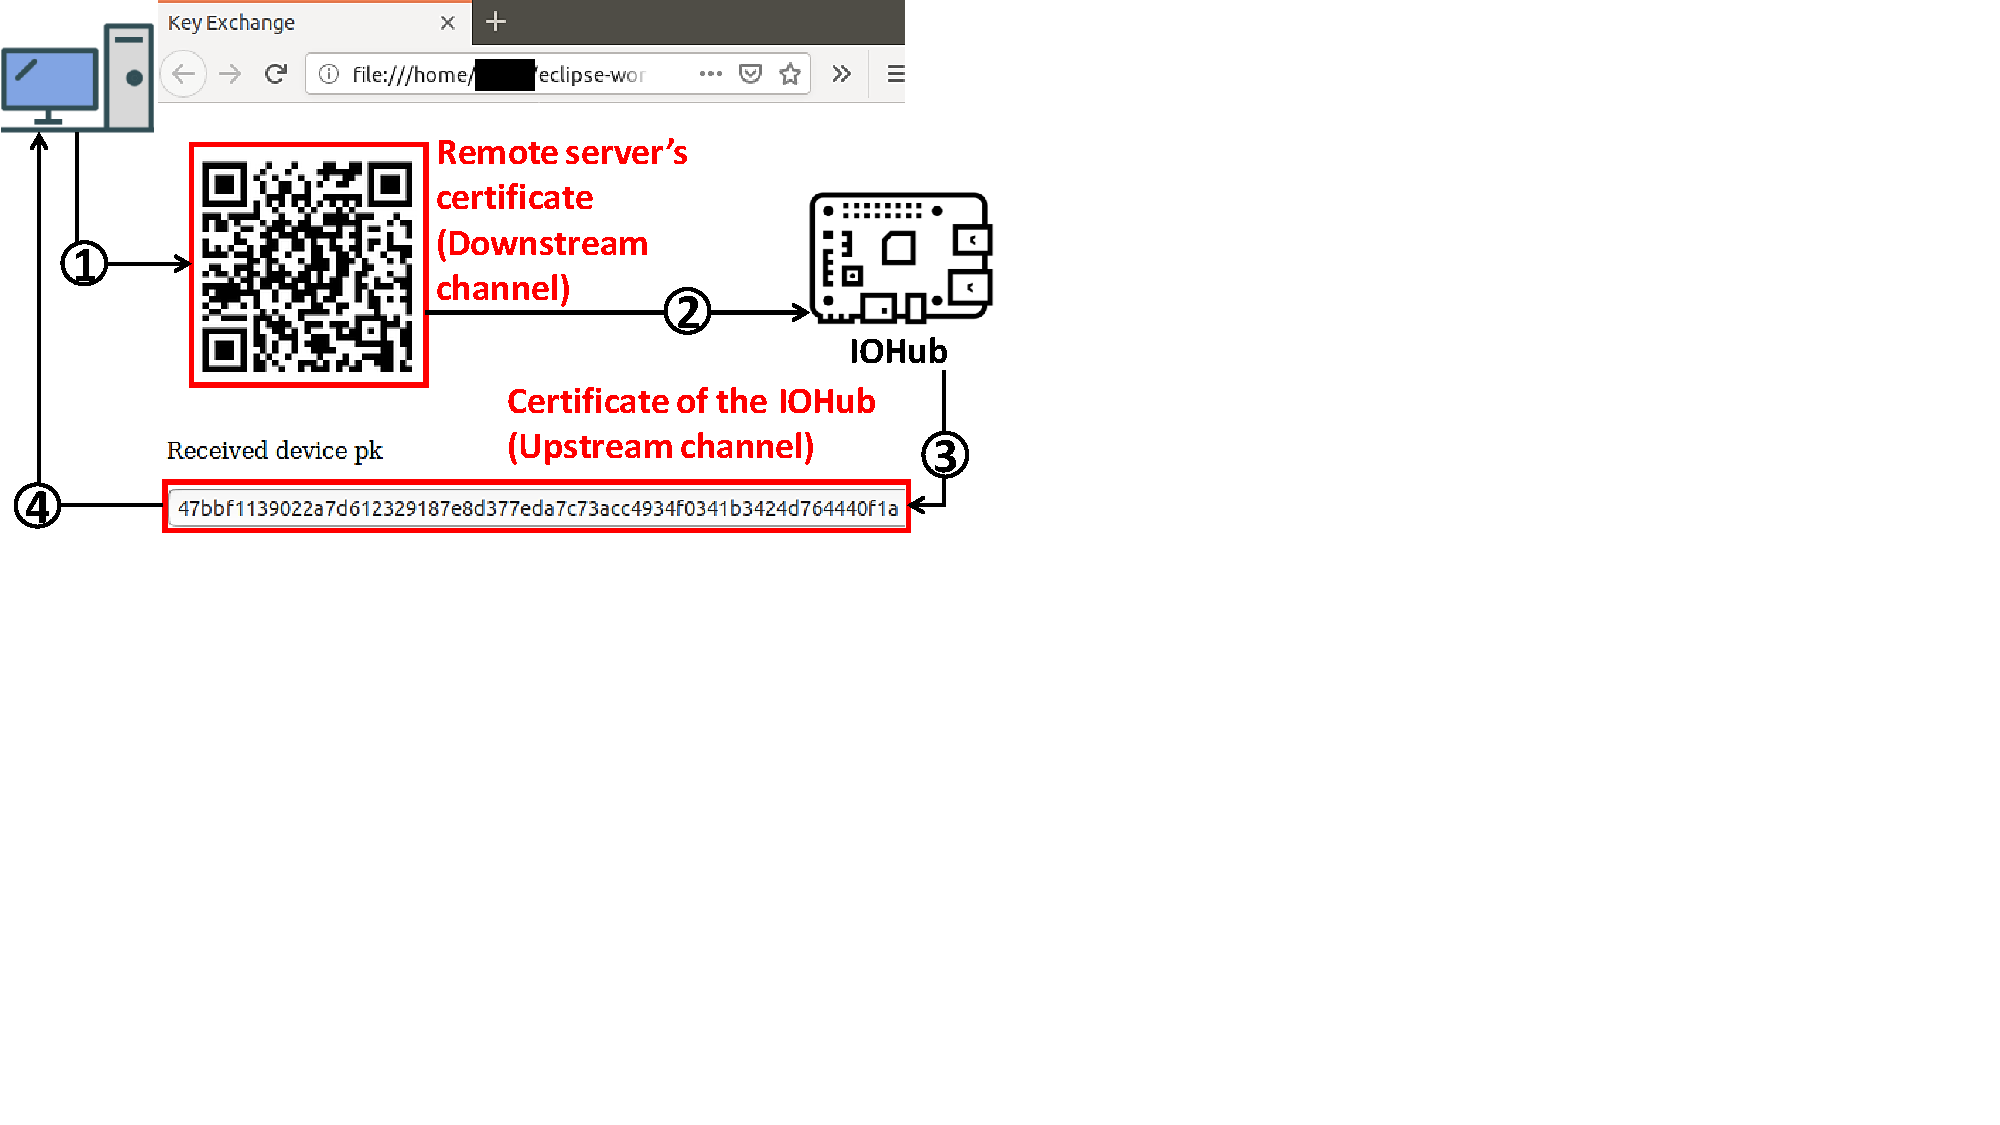
\includegraphics[trim={0 10cm 17cm 0}, clip, width=0.8\linewidth]{chapters/ProtectIOn/images/keyExchange_1.pdf}
\caption[Establishing \tls between \device and the remote server]{\textbf{Establishing \tls between \device and the remote server.} A snapshot of the key exchange web page that is used to communicate the public certificates of the \device and the remote server.}
%\spacesave
\label{fig:keyExchange}
\centering
\end{figure} 

\subsection{Establishing \tls}
\label{sec:prototype:impl:tls}
%
For the IO confidentiality, the \device and server create a \tls channel. When the user opens up a secure webpage, key exchange is the first step that takes place. We assume that the remote server already has the \device's certificate, or some offline registration takes place. An instance of the key exchange protocol of \name is illustrated in Figure~\ref{fig:keyExchange}. The flow of the key exchange mechanism is as the following:
%\vspace{-10pt}
\begin{enumerate}
  \item[\one] The server delivers a web page with a QR code that encodes the signed public key of the server (server hello in TLS). 
  \item[\two] The device captures every frame until it detects a QR code. Then, it decodes the QR code and verifies the public key and derives the shared secret using Diffie-Hellman protocol~\cite{blake1998authenticated}. 
  \item[\three] The device then sends its signed public certificate to the host, which forwards it to the server.
  \item[\four] The remote server gets the signed certificate from the \device, verifies it, and finally derives the shared secret.
\end{enumerate}

\begin{figure}[t]
\centering
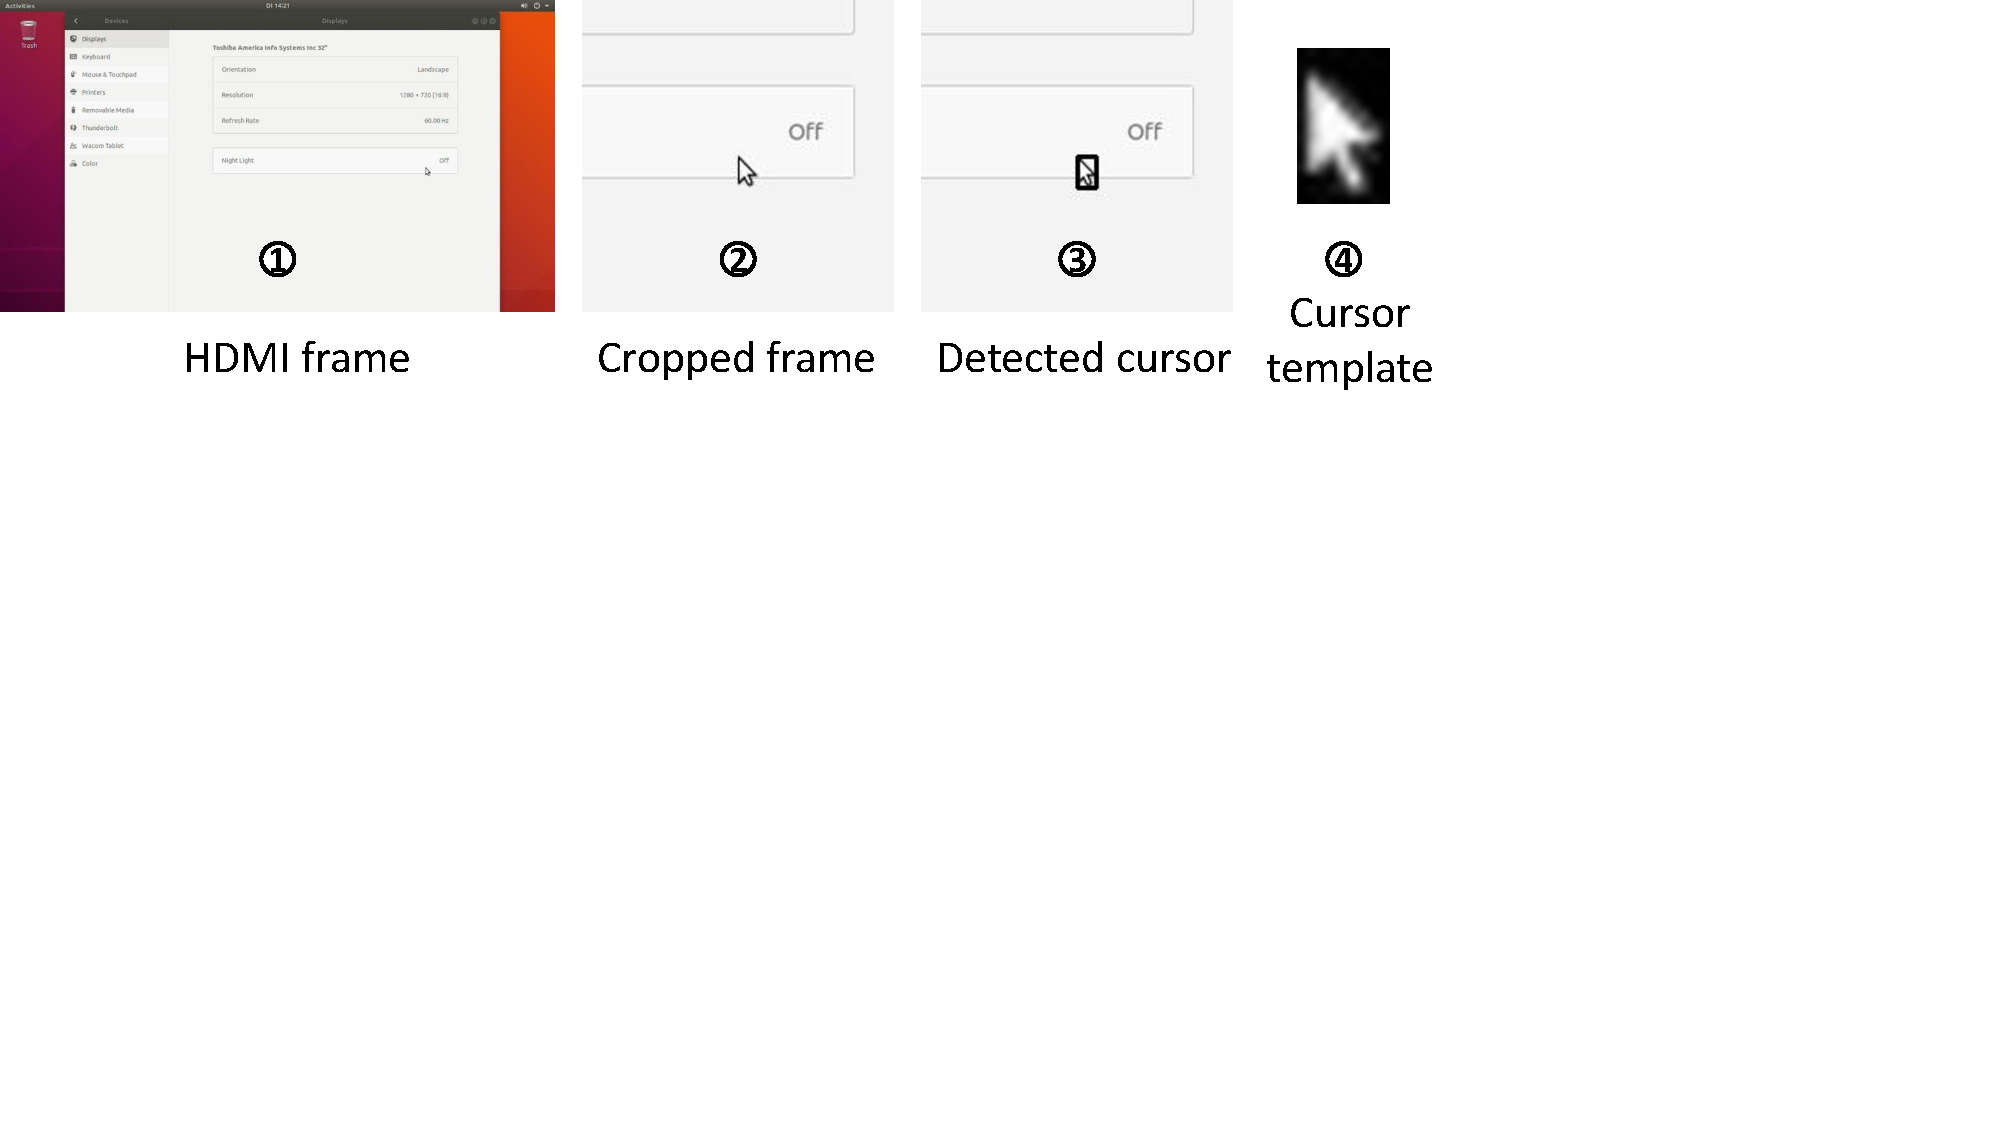
\includegraphics[trim={0 12cm 10cm 0}, clip, width=\linewidth]{chapters/ProtectIOn/images/cursorDetect.pdf}
\caption[Cursor detection on the HDMI frame]{\textbf{Cursor detection on the HDMI frame.} The figure shows \name mouse pointer tracking. \one shows the captured HDMI frame captured by B101 HDMI to CSI bridge. \two shows the cropped HDMI frame based on the mouse position received by the \device. \three shows the detected mouse pointer. For testing, we program the \device to put a rectangle around the pointer. \four shows one of the pointer templates that we used in our OpenCV routine.}
%\spacesave
\label{fig:cursorDetect}
\centering
\end{figure} 


\subsection{HID Drivers}
We use Arduino prototype development board as the HID drivers. Figure~\ref{fig:prototype} shows an Arduino Due, and a Zero board where the Due connects to the HIDs via the native USB port and the Zero relays the HID data to the Raspberry Pi (RPi). The Due and the Zero boards are connected over $I^2C$ interface. As both Due and Zero only have one native USB port on each of them, we were forced to use two boards as an HID interceptor and relay. The Zero relays the HID signals both to the connected host (over native USB) and to the RPi (over serial interface). The connection from the Zero to the host is one way and emulates a composite HID. While the connection between the Zero and the RPi is bidirectional. The HID drivers are implemented using the native Arduino \texttt{keyboard} and \texttt{mouse} library. On the RPi, no HID drivers were needed as the RPi receives processed HID data from the Zero (for the pointer: displacement over x and y-axis and for keyboard, ASCII characters).


\subsection{HDMI Interceptor, Relay and Overlay}
The RPi along with the Auvidea B101 HDMI to CSI bridge, acts as the HDMI interceptor and relay. The B101 board converts HDMI signals from the host as a camera input (via the CSI interface) to the RPi. This allows the RPi to access the HDMI frames as a stream of JPEG frames. The HDMI out of the RPi acts as the relay that connects to the monitor. On the RPi, we use Picamera API~\cite{picamera} to access the HDMI frames. The B101 is capable of processing 25 frames at 1080p resolution. Hence, this is the hardware bottleneck of our implementation. However, the upcoming B112 board
%\footnote{still in development: \url{https://auvidea.eu/showcase/}.} 
could solve this performance issue.

On the RPi, the overlay and HDMI out is implemented using Java SWT. Using SWT, we create a full-screen window that is shown on the monitor. The SWT class polls the HDMI frames and process them as individual JPEG images via the \texttt{BufferedImage} class. This allows the overlays to be drawn on the HDMI images efficiently. The Java program uses a QR code interpreter to extract the UI specification. Based on the UI specification, it creates the geometrical shapes (corresponding to the UI elements) and draw them on the frames. In the current implementation of the \name, the UI elements such as button, text-field, radio button etc. are preloaded in the \device memory. Note that the current implementation of \device is based on the RPi. But one could implement such functionality on an FPGA, reducing the TCB even more. 


\subsection{Mouse Pointer Tracking}
The pointer tracing is also executed in the aforementioned Java program using simple object detection technique suppled by the OpenCV API. Figure~\ref{fig:cursorDetect} shows one screenshot of the pointer detection. The Figure shows the entire HDMI frame, the cropped frame of resolution $200 \times 200$ px (based on the mouse input data), the detected pointer in the cropped frame and the cursor template that is used by the object detection algorithm.



